% !TeX root = ../../../book.tex

\subsection{其他计数对象}

\subsubsection*{$[k]$ 中的 $n$-元组}

扑克牌是很好的、标准的物理计数对象。大多数人都很熟悉扑克牌,因为每张牌都有两个属性 --- 花色和点数 --- 这使得我们可以设计许多有趣的组合问题。一个更``抽象''的标准计数对象例子是具有指定长度的自然数列表。我们将做出以下定义,以便我们能够简洁地引用这些集合。

\begin{definition}
    给定 $n,k \in \mathbb{N}$,则
    \[T_{k,n} = [k]^n = \{(a_1, a_2, \dots , a_n) \mid \forall i \centerdot a_i \in [k]\}\]
    也就是说,$T_{k,n}$ 是所有元素属于 $[k]$ 的 $n$-元组的集合。
\end{definition}

注意:我们选择字母 $T$ 是因为这些对象是 \emph{$n$-元组 (Turple)},即长度为 $n$ 的有序列表。需要指出的是,当 $k$ 是一个较小的数值,如 $2$ 或 $3$ 时,通常会把集合 $[k]$ 替换为 $[k - 1] \cup \{0\}$。例如,二进制 $n$ 元组的概念在数学中非常常见,部分原因是它在计算机科学中的广泛应用。因此,当 $k = 2$ 时,常常考虑长度为 $n$ 的有序列表,其元素来自集合 $\{0, 1\}$,而不是 $\{1, 2\}$。由于我们关注的是这些集合的组合特性(例如``具有属性 $P$ 的序列有多少?''),实际上选择哪种约定并不重要。事实上,通过在基础集合 $[k]$ 和 $[k - 1] \cup \{0\}$ 之间建立双射,可以轻松证明
\[|T_{k,n}| = |[k]^n| = k^n = |([k - 1] \cup \{0\})^n|\]
这部分留给你来完成$\smiley{}$

在下一节中,我们会看到许多计数论证,都可以通过确定适当的 $k$ 和 $n$ 以及有序列表的附加属性来方便地表达。现在,让我们研究几个简单的例子并探索一些应用。在每个例子中,我们会研究子集 $S \subseteq T_{k,n}$,这些子集的元素具有某些特定属性;具体来说,我们会通过计算 $S$ 中元素的数量来得到 $|S|$。我们将从一些非常简单的例子开始,然后逐步探讨更具挑战性的例子。本节中的练习将进一步深入这些概念。\\

\begin{example}
    设 $n=4, k=3$

    \begin{enumerate}[label=(\arabic*)]
        \item $|T_{3,4}|$ 是多少?\\
              要计算 $T_{3,4}$ 的所有元素,我们可以通过一个四步过程来构建这个集合,其中第 $i$ 步对应于选择 $4$-元组中的第 $i$ 个元素。在每一步中,我们有 $3$ 个选项(每个元素是 $\{1, 2, 3\}$ 之一),因此乘法原理告诉我们 $T_{3,4}$ 共有 $3 \cdot 3 \cdot 3 \cdot 3 = 3^4 = 81$ 个元素。(注意:请参见练习 \ref{},要求证明 $|T_{n,k}| = n^k$ 的一般情况。)
        \item $T_{3,4}$ 的元素中有多少不包含 $1$?\\
              要计算 $T_{3,4}$ 中没有 $1$ 的元素数量,我们可以通过限制每一步的选项来简化四步过程。具体来说,$T_{3,4}$ 中没有 $1$ 的元素其 $4$ 个位置只能从集合 $\{2, 3\}$ 中选择。因此,根据乘法原理,有 $2 \cdot 2 \cdot 2 \cdot 2 = 2^4 = 16$ 个这样的元素。
        \item $T_{3,4}$ 的元素中有多少只包含一个 $1$?有多少包含两个 $1$?有多少包含三个 $1$?有多少包含四个 $1$?\\
              如何计算 $T_{3,4}$ 中恰好含有一个 $1$ 的元素数量?是否可以使用与上一问相同的思路?答案是不完全可以!在这个过程中,每一步的可选项数量可能会发生变化,这取决于是否已经在 $4$-元组中放置了一个 $1$。我们需要找到一种新的方法。相反,我们可以考虑先在 $4$-元组中的某个位置放置一个 $1$,然后用 $\{2, 3\}$ 中的元素填充剩余的位置。具体来说,我们可以通过以下四个步骤构建一个恰好含有一个 $1$ 的 $4$-元组:
              \begin{enumerate}[label=(\alph*)]
                  \item 选择四个位置中的一个来放置数字 $1$:有 $\big({4 \atop 1}\big)=4$ 种方法。\\
                        然后,对于剩下的三个空位,从左到右依次填入。
                  \item 对于第一个空位,从 $\{2, 3\}$ 中选择一个元素:有 $2$ 种方法。
                  \item 对于第二个空位,从 $\{2, 3\}$ 中选择一个元素:有 $2$ 种方法。
                  \item 对于第三个空位,从 $\{2, 3\}$ 中选择一个元素:有 $2$ 种方法。
              \end{enumerate}
              因此,$T_{3,4}$ 中共有 $4 \cdot 2^3 = 32$ 个这样的元素。
    \end{enumerate}

    或许我们在这个论证中显得有些啰嗦。其实可以简化为两个步骤:首先确定 $1$ 的位置,然后从 $\{2, 3\}$ 中选择余下 $3$ 个位置的值。这只是表述上的不同,本质上证明的是同一事实。我们提供这些额外的细节是为了确保你能理解我们的论证和其中的基本原理,这将帮助你将这些思路应用到你自己的证明中。

    我们可以用类似的方法来计算 $T_{3,4}$ 中恰好有两个 $1$ 的元素数量。唯一的区别在于步骤 1:我们需要从 $4$ 个位置中选择 $2$ 个位置来放置 $1$。这有 $\big({4 \atop 1}\big)$ 种选择方法。然后,剩余两个位置需要从 $\{2, 3\}$ 中选择。因此,$T_{3,4}$ 中有
    \[\begin{pmatrix}
            4 \\
            2
        \end{pmatrix} \cdot 2^2 = 24\]
    个这样的元素。

    我们留给你来验证 $T_{3,4}$ 中恰好有三个 $1$ 的元素有 $8$ 个,恰好有四个 $1$ 的元素有 $1$ 个。我们也留给你来验证并解释为什么 $16 + 32 + 24 + 8 + 1 = 81$ 是合理的。(挑战性问题:你能将这个结果推广到任意 $n$ 和 $k$ 吗?)
\end{example}

\begin{example}
    设 $n \ge 3$。我们来计算以下几种二进制 $n$-元组的数量:
    \begin{enumerate}[label=(\alph*)]
        \item 恰好有三个 $1$;
        \item 至少有三个 $1$;
        \item 有偶数个 $1$。
    \end{enumerate}

    我们这里讨论的集合是 $\{0, 1\}^n$,即所有元素为 $\{0, 1\}$ 的 $n$-元组。(注意,这并不是前面定义的集合 $T_{2,n}$,但我们已经解释了如何在这两个集合之间建立一个双射。)

    要解答问题 (a),我们使用与前一个例子相同的方法。首先,从 $n$ 个位置中选择 $3$ 个位置放置 $1$;然后,用 $0$ 填充剩下的 $n-3$ 个位置。第一步有 $\big({n \atop 3}\big)$ 种选择方法,第二步是确定的(即只有 $1$ 种方法),所以共有 $\big({n \atop 3}\big)$ 种二进制 $n$-元组恰好有三个 $1$。(注意:我们规定 $n \ge 3$ 是为了确保答案不为零。如果 $1 \le n \le 2$,那么显然不可能有这样的元组!确实,这也验证了当 $\ell > n$ 时,$\big({n \atop \ell}\big) = 0$。)

    要解答问题 (b),我们使用与解答问题 (a) 相同的方法,但将其从 $3$ 推广到任意自然数个 $l$。具体来说,我们可以计算出恰好有 $\ell$ 个 $1$ 的二进制 $n$-元组的数量,方法如下:先选择 $n$ 个位置中的 $\ell$ 个填充 $1$,然后将其余位置填充 $0$。为了至少包含三个 $1$,我们需要恰好有三个 $1$,或者四个 $1$……依此类推,直到 $n$ 个 $1$。更严格地说,对于每个在 $3$ 到 $n$(包括 $3$ 和 $n$)之间的 $\ell$,设 $A_\ell$ 为恰好有 $\ell$ 个 $1$ 的二进制 $n$-元组集合。每个至少有三个 $1$ 的二进制 $n$-元组都恰好属于一个 $A_l$ 集合。因此,我们得到了要计算的元组集合的一个\emph{划分},每部分包含特定数量的 $1$。根据加法原理,我们最终得到的数量为
    \[\sum_{\ell = 3}^{n} |A_\ell| = \sum_{\ell = 3}^{n} \begin{pmatrix}
            n \\
            \ell
        \end{pmatrix}\]
    你可能会想,用求和符号表示的答案是否\emph{可以接受}。从某种意义上讲,它是可以接受的;就在 $10$ 分钟前,我们还不知道有多少个至少有三个 $1$ 的二进制 $n$-元组,现在我们对这个数字有了更好的了解。然而,上述解决方案更像是一种找到精确数字的方法。如果有人在街上问你,``快!告诉我至少有三个 $1$ 的二进制 $n$-元组的数量!'',你会怎么做?你会说,``等等,我只需要通过分别计算每一项并相加来求和……''这并不理想,是吧?如果有一个简单形式的解会更好、更方便;也许我们可以把它写成一个二项式系数,或者两个或三个或某些较小数量的二项式系数的和、差、积或商。这样,无论 $n$ 是多少(即无论它有多大),我们都知道可以通过几个简单步骤高效地计算出答案;此外,我们希望步骤数量不会随着 $n$ 的增加而增加。用上述求和形式,求和项的数量会随着 $n$ 的增加而增加。这并不理想。

    我们将细节部分留给您来验证和解释,但我们声称,通过应用加法原理,可以对所有二进制 $k$-元组进行适当的划分,从而证明
    \[2^n = \begin{pmatrix}
            n \\
            0
        \end{pmatrix} + \begin{pmatrix}
            n \\
            1
        \end{pmatrix} + \begin{pmatrix}
            n \\
            2
        \end{pmatrix} + \sum_{\ell = 3}^{n} \begin{pmatrix}
            n \\
            \ell
        \end{pmatrix}\]
    实际上,这个等式的证明涉及到我们将在下一节讨论的技术,不过我们相信你可以理解这个等式中的术语及其成立的原因。不过,我们要强调的是,通过整理该等式,我们可以得到一个在某种意义上形式更好的解:
    \[\sum_{\ell = 3}^{n} \begin{pmatrix}
            n \\
            \ell
        \end{pmatrix} = 2^n - \begin{pmatrix}
            n \\
            0
        \end{pmatrix} - \begin{pmatrix}
            n \\
            1
        \end{pmatrix} - \begin{pmatrix}
            n \\
            2
        \end{pmatrix}\]
    看看我们的成果!无论 $n$ 多大,我们只需评估四项。这里\emph{固定}数目是关键。事实上,我们非常喜欢这种形式的解,所以给它取了个名字:\textbf{闭合解}。其特点是没有``多余''的求和,无论所包含的变量值是多少,项的数量固定。

    通常,在解决组合数学问题时,我们总是尽量寻找\textbf{闭合解}。有时候,我们很容易想到一个非闭合(有些人可能会称之为``开放'')形式的解,但将其简化为闭合形式可能需要一些巧妙的思考。在这个具体例子中,我们观察到所有二进制 $n$-元组可以分类为恰好有零个 $1$、一个 $1$、两个 $1$ 或至少三个 $1$。这种闭合解不仅使我们能够更快、更容易地计算表达式,还能提供对问题底层结构的更多见解。因此,我们总是追求闭合解。

    现在,我们不要忘记问题 (c)!为了回答它,我们采用与 (b) 类似的技术,将具有偶数个 $1$ 的二进制 $n$-元组集合划分为恰好有零个 $1$(记住,$0$ 是偶数!)、恰好有两个 $1$、恰好有四个 $1$,等等。不过,我们必须注意上限,因为 $n$ 本身不一定是偶数!回想一下向下取整函数,它将一个数向下舍入到不大于该数的最大整数;例如 $\lfloor 5.7 \rfloor = 5$。考虑到这一点,我们声称有
    \[\sum_{\ell=0}^{\lfloor n/2 \rfloor} \begin{pmatrix}
            n \\
            2\ell
        \end{pmatrix}\]
    个二进制 $n$-元组具有偶数个 $1$。我们将解释该声明的机会留给你。试着向你的朋友证明并说服他们这是正确的。不要放弃,直到他们完全信服!我们将放弃寻找其\emph{闭合解},因为这超出了我们的能力……看看你能从这个求和中推断出什么!当 $n$ 是偶数时会发生什么?当 $n$ 是奇数时又会发生什么?是否有类似的求和可以将这个表达式联系起来?你能得出什么结论?
\end{example}

\begin{example}
    计算 $1$ 成对出现的二进制 $4$-元组的数量。举个例子,我们会把 $(1, 1, 0, 0)$ 和 $(1, 1, 1, 1)$ 算进去,但不会包括 $(1, 0, 1, 1)$ 或 $(0, 1, 1, 1)$。然后,我们将这个方法扩展到二进制 $5$-元组,看看能否找到一个通用模式。

    如果一个 $4$-元组中的 $1$ 成对出现,那么总共有 $0$ 个、$2$ 个或 $4$ 个 $1$。我们定义集合 $S_0$、$S_2$ 和 $S_4$,分别表示 $1$ 成对出现且总数为 $0$ 个、$2$ 个或 $4$ 个的二进制 $4$-元组。(注意:$S_2$ 并不是指只有两个 $1$ 的二进制字符串,因为那样会错误地包括像 $(1, 0, 1, 0)$ 这样的字符串。)这些集合构成了我们要计数的所有元素的划分,所以我们只需要计算这三个集合中元素的数量,然后应用加法原理将它们相加即可。
    \begin{itemize}
        \item 为了得到 $|S_0|$,我们需要计数没有 $1$ 的二进制 $4$-元组,这样的元组只有一个:$(0, 0, 0, 0)$。
        \item 为了得到 $|S_2|$,我们需要计数有两个连续 $1$ 且剩余位置由 $0$ 填充的二进制 $4$-元组。手动列出这些情况,
              \[(1, 1, 0, 0) \qquad (0, 1, 1, 0) \qquad (0, 0, 1, 1)\]
              显然只有 $3$ 个这样的元组。(你能找到一个更巧妙的论证来解释为什么只有 $3$ 个吗?我们会在研究 $5$-元组时再次回到这个问题。)
        \item 为了得到 $|S_4|$,我们需要计数有四个 $1$ 的二进制 $4$-元组。显然 $(1, 1, 1, 1)$ 是唯一的答案。
    \end{itemize}
    根据加法原理,有 $ 1 + 3 + 1 = 5$ 个 $1$ 成对出现的二进制 $4$-元组

    要回答关于 $5$-元组的问题需要一些巧妙的方法。我们将定义相同的集合 $S_0$、$S_2$ 和 $S_4$,但将 $4$-元组修改为 $5$-元组。这 $3$ 个集合仍然构成我们要计算的二进制 $5$-元组的一个划分。只需计算每个集合中元素的数量,再应用加法原理即可。
    \begin{itemize}
        \item $|S_0|=1$,因为只有一个不包含 $1$ 的 $5$-元组:$(0, 0, 0, 0, 0)$。
        \item 为了得到 $|S_2|$,我们可以手动写出所有情况,但最好能提出一个可以轻松适用于 $k$-元组的方法,其中 $k \in \mathbb{N}$。为了有一对 $1$ 并且其余位置由 $0$ 填充,我们可以将``$1, 1$''视为一个整体,放置在三个 $0$ 之间。因此,我们实际上是在计算如何将一个特殊整体放置到长度为 $4$ 的有序列表中,然后用另一个固定元素确定性地填充剩余位置。当然,有 $4$ 种方法可以做到这一点,手动写出这些情况可以验证这一点。(实际上我们注意到,连续的一对 $1$ 是由元组中\emph{第一个} $1$ 的索引确定的;该索引可以是 $\{1, 2, 3, 4\}$ 中的任意一个,所以有 $\big({4 \atop 1}\big) = 4$ 种选择。)
        \item 上面的方法同样适用于 $|S_4|$ 的情况。在这里,我们有两对连续的 $1$,因此可以将每对``$1,1$''看作一个整体。这样,我们实际上有两个``$1,1$''和一个 $0$ 需要放入长度为 $3$ 的有序列表中。由于两个``$1,1$''是相同的,我们可以通过选择这两个``$1,1$''的位置来计算有序列表的数量。因此,有 $\big({3 \atop 2}\big) = 3$ 种排列方式。(同样,我们也可以通过选择 $0$ 的位置来计算,即 $\big({3 \atop 1}\big) = 3$ 种选择。)
    \end{itemize}
    因此,有 $1 + 4 + 3 = 8$ 个 $1$ 成对出现的二进制 $5$-元组
\end{example}

\subsubsection*{字母表与单词}

从 $[n]$ 中抽取元素组成 $k$-元组的概念与从给定\emph{字母表}中构造\emph{单词}的概念非常相似。实际上,从数学的角度讲,这两个概念是\emph{等价的},并没有什么新的内容!不过,这样的表述可以使用不同的术语,并且与一些``现实世界''的概念和问题相关联。出于这个原因,以及你可能会觉得某种表述更容易理解,我们在本小节中介绍这一点,并与前一小节的内容进行联系。

我们将通过一些例子来介绍和解释本小节的思想。在每个例子中,我们会给定一个字母表,其元素是我们可以用来构造单词的字母。不过,这里的``单词''实际上是指从给定字母表中抽取的任何有序字母串。例如,在第一个例子中,我们使用标准的英文字母表;在这种情况下,\verb|ZPQ| 是一个完全可以接受的三字母单词(不过要发音可能有点困难!)。我们允许这种泛化的主要原因是为了避免任何语义学或词源学的争论,例如 \verb|REALISE| 是否应该是 \verb|REALIZE| 的一个可接受变体,或者 \verb|ZZZ| 是否真的算作一种拟声词。这意味着我们必须剥离``单词''这个词的一些含义,只将其视为由字母组成的字符串,除了字母及其顺序外没有其他固有意义。\\

\begin{example}
    让我们以标准的 $26$ 个英文字母为例。
    \begin{enumerate}
        \item 用这个字母表可以组成多少个 $3$ 字母单词?\\
              这相当于问 $T_{26,3}$。我们有 $26$ 个字母,并希望组成长度为 $3$ 的有序列表。通过将集合 $\{A, B, C, \dots , Z\}$ 和 $[26]$ 之间建立一个双射(这实际上是你小时候可能玩过的替换密码),我们可以严格地证明这个问题相当于问 $|T_{26,3}|$ 是多少。\\

              即便不进行这种连接,我们也可以通过观察发现构造一个 $3$字母单词相当于一个 $3$ 步过程(从左到右填入 $3$ 个字母),每步有 $26$ 个选项,从而轻松地计算出 $3$ 字母单词的数量。因此,有 $26^3$ 个 $3$ 字母单词。
        \item 可以组成多少个 $4$ 字母单词?\\
              按照前面的逻辑,有 $26^4$ 个 $4$ 字母单词。
        \item 可以组成多少个 $n$ 字母的单词?\\
              这个问题留给你来解答。$\smiley{}$
        \item 有多少以元音开头的 $4$ 字母单词?\\
              注意:我们认为 $\{A,E,I,O,U\}$ 是元音(即使字母歌可能告诉你 $Y$ 是元音,但我们这里不包括 $Y$)。考虑到这一点,我们可以修改构造 $4$ 字母单词的过程,以保证第一个位置是元音。完成这一步有 $5$ 种方法,接下来的 $3$ 步每步有 $26$种选择。因此,有 $5 \cdot 26^3$ 个以元音开头的 $4$ 字母单词。
        \item 有多少最多有 $2$ 个辅音的 $4$ 字母单词?\\
              辅音是非元音,因此根据我们的定义,字母表中有 $26 - 5 = 21$ 个辅音。最多有两个辅音意味着我们有正好 $0$ 个或正好 $1$ 个或正好 $2$ 个辅音,因此我们可以将这些单词划分为三个集合,$S_0, S_1, S_2$,并分别计数。通过应用乘法法则,我们发现
              \begin{align*}
                  |S_0| & = 5^4                                                     \\
                  |S_1| & = \begin{pmatrix} 4\\1 \end{pmatrix} \cdot 21 \cdot 5^3   \\
                  |S_2| & = \begin{pmatrix} 4\\2 \end{pmatrix} \cdot 21^2 \cdot 5^2
              \end{align*}
              因此,有
              \[5^4 +  4 \cdot 21 \cdot 5^3 + \begin{pmatrix} 4\\2 \end{pmatrix} \cdot 21^2 \cdot 5^2\]
              个最多有两个辅音的 $4$字母单词。(挑战性问题:有多少个 $4$字母单词至少有三个辅音?用这里的结论和 $26^4$ 给出一个声明。)\\

              关于 $S_2$ 的以下论点有什么问题:通过选择两个辅音来构造一个正好有两个辅音的四字母单词,然后为第一个辅音选择一个位置,然后为第二个辅音选择一个位置,然后用元音填充剩下的两个位置,从而得到
              \[\begin{pmatrix} 21\\2 \end{pmatrix} \cdot 4 \cdot 3 \cdot 5^2\]
              个这样的单词。\\

              仔细思考这个问题。记住,这些``找出错误''问题不仅仅是让你识别出有错误,还要解释为什么是错误的以及如何修正。
        \item 有多少由 $4$ 个不同字母组成的 $4$ 字母单词?\\
              我们可以不加思索地通过描述一个从左到右填写四个字母的四步过程来回答这个问题,并在每一步减少一个选项。因此,有
              \[26 \cdot 25 \cdot 24 \cdot 23\]
              个由四个不同字母组成的四字母单词。\\

              这看起来是不是很熟悉?回顾我们定义\emph{排列}的方法。这正是我们在这里使用的思路!从一个包含 $26$ 个元素的集合中,我们想要构造一个长度为 $4$ 且没有重复的有序列表,即从包含 $26$ 个元素的集合中选取 $4$ 个元素进行排列。我们推导出的公式告诉我们有
              \[\begin{pmatrix} 26\\4 \end{pmatrix} \cdot 4! = \frac{26!}{4! \cdot 22!} 4! = \frac{26!}{22!} = 26 \cdot 25 \cdot 24 \cdot 23\]
              个这样的排列。这个例子告诉我们:通过利用先前定义的术语和推导的公式,并将当前问题与这些概念联系起来,我们可以快速找到问题的解。
        \item 有多少 $4$ 字母单词恰好有一个字母重复两次?\\
              要构造这样的单词,我们需要知道哪个字母重复了两次,以及它的两个位置分别在哪里,还需要确定单词中另外两个字母。因此,我们可以分三步来进行:
              \begin{enumerate}[label=(\arabic*)]
                  \item 选择要重复的字母;
                  \item 在四个位置中选择两个放置该字母;
                  \item 在剩下的两个位置放置剩下的 $25$ 个字母中的两个。
              \end{enumerate}
              因此,有
              \[\begin{pmatrix} 26\\1 \end{pmatrix}\begin{pmatrix} 4\\2 \end{pmatrix}\begin{pmatrix} 25\\2 \end{pmatrix} \cdot 2!\]
        \item 有多少 $5$ 字母单词恰好有两个字母各自重复两次?\\
              按照与之前例子类似的逻辑,我们可以进行以下步骤:
              \begin{enumerate}[label=(\arabic*)]
                  \item 选择两个要重复的字母;
                  \item 在 $5$ 个空位中选择两个位置放第一个按字母顺序排列的重复字母;
                  \item 在剩下的 $3$ 个位置中选择两个位置放第二个按字母顺序排列的重复字母;
                  \item 在剩余的 $24$ 个字母中选择一个字母填充最后一个位置。
              \end{enumerate}
              因此,有
              \[\begin{pmatrix} 26\\2 \end{pmatrix}\begin{pmatrix} 5\\2 \end{pmatrix}\begin{pmatrix} 3\\2 \end{pmatrix}\begin{pmatrix} 24\\1 \end{pmatrix}\]
    \end{enumerate}
\end{example}

\begin{example}
    有多少种排列可以让字母 \verb|U| 和 \verb|ME| 在一起?$\smiley{}$

    你可能会想到用``排除法''来解决这个问题,也就是说,你可能会尝试计算所有不把字母 \verb|U| 放在字母 \verb|ME|(按这个顺序)旁边的排列。你可以试试看会得到什么结果。然而,我们将提出一种不同的方法,并且我们认为这种方法更简洁。该方法的思路在其他问题中也会用到,归结起来就是将两个字母的单词 \verb|ME| 视为一个整体,就像其他单个字母一样。

    换个角度来看问题,与其问从给定字母表中有多少种类型的单词,我们不妨问给定单词有多少种排列组合(即\emph{异序词})。在考虑这些问题时必须小心,因为当字母重复时,情况会变得复杂!例如,单词 \verb|A| 有多少种异序词?单词 \verb|AAAAA| 呢?单词 \verb|AABBBCCCCDD| 呢?没错!你应该抓到了我们想要表达的核心观点。
\end{example}

\begin{example}
    让我们从一个简单的例子入手。单词 \verb|HEART| 有多少个异序词?记住,我们将字母的所有排列都视为有效单词,所以不要用拼字游戏的思维考虑这个问题 $\smiley{}$。(顺带一提,在拼字游戏中,这个问题的答案是 $4$ --- \verb|HEART, HATER, EARTH, RATHE|。)由于这个单词的每个字母都\emph{不同},答案很简单:只需计算 $5$ 个字母的全排列即可。因此,\verb|HEART| 有 $5! = 120$ 个异序词。

    \verb|APPLE| 有多少个异序词呢?注意到字母 \verb|P| 出现了两次,所以我们不能简单地考虑五个元素的全排列。如果那样做,每个单词实际上都会重复计算两次;也就是说,\verb|APPLE| 这个单词会被重复计数。你能看出这两个单词有什么不同吗?我们只是交换了两个 \verb|P|!显然,它们是相同的单词,所以我们在考虑排列时需要把这一点考虑进去。

    我们该怎么处理这个问题呢?一个有用的技巧是给重复的 \verb|P| 打上``标签''。从左到右读取 \verb|APPLE|,我们称第一个 \verb|P| 为 $\mathtt{P_1}$,第二个 \verb|P| 为 $\mathtt{P_2}$。这将帮助我们理清重复的排列。现在,我们有五个不同的元素 --- $\mathtt{A, P_1, P_2, L, E}$ --- 所以我们可以考虑这些元素的所有 $5!$ 个排列。我们知道这样会导致重复计数,所以我们需要弄清楚重复计数的程度。定义 $G$ 为 \verb|APPLE| 的异序词集合(我们正在尝试计算 $|G|$),并定义 $M$ 为上述五个不同元素的全排列集合。$|G|$ 和 $|M|$ 之间有什么关系呢?

    要回答这个问题,我们可以考虑从 $G$ 的元素构造 $M$ 的元素。具体来说,我们可以通过先取 $G$ 的一个元素(\verb|APPLE| 的一个异序词),然后给 \verb|P| 打上标签来构造 $M$ 的任意一个元素(五个不同元素的全排列)。然而,这样并不能生成 $M$ 的所有元素。为此,我们必须从 $G$ 的元素中构造两个元素;具体来说,我们需要给 \verb|P| 打上标签,然后考虑单词中 \verb|P| 的两种排列方式。让我们看一个例子:
    \begin{itemize}
        \item 取 $G$ 中的一个元素,比方说 \verb|PAPEL|。
        \item 从左到右给 \verb|P| 打上标签:$\mathtt{P_1AP_2EL}$。
        \item 构建两种 \verb|P| 的排列,并将这两个词都作为 $M$ 的元素:$\mathtt{P_1AP_2EL} \in M$ 且 $\mathtt{P_2AP_1EL} \in M$。
    \end{itemize}
    由于两个 \verb|P| 有 $2! = 2$ 种排列方式,我们已经证明了 $|G| \cdot 2! = |M|$。我们描述了一个生成 $M$ 元素的两步过程并应用了乘法原理。因此,我们可以通过整理这个方程来得到我们要寻找的数量:
    \[|G| \cdot 2! = |M| \implies |G| = \frac{|M|}{2!} = \frac{5!}{2!} = 60\]

    让我们来看一个稍微复杂一点的例子,计算单词 \verb|COMBINATORICS| 的异序词。我们将使用与前一个例子相同的策略,通过标记重复的字母,将异序词与 $13$ 个不同元素的全排列联系起来。我们定义 $G$ 为单词 \verb|COMBINATORICS| 的所有异序词集合,$M$ 为由 ${\mathtt{C_1O_1MBI_1NATO_2RI_2C_2S}}$ 中 $13$ 个不同元素组成的全排列集合。我们可以用四个步骤来生成 $M$ 中的元素:
    \begin{itemize}
        \item 取 $G$ 中的元素从左到右标记重复字母:有 $|G|$ 种方式。
        \item 排列重复的 \verb|C|:有 $2!$ 种方法。
        \item 排列重复的 \verb|O|:有 $2!$ 种方法。
        \item 排列重复的 \verb|I|:有 $2!$ 种方法。
    \end{itemize}
    因此,根据乘法原理,我们可以得到
    \[|M| = |G| \cdot 2! \cdot 2! \cdot 2! \implies |G| = \frac{|M|}{2! \cdot 2! \cdot 2!} = \frac{13!}{2! \cdot 2! \cdot 2!}\]
    你可能会好奇,为什么我们会写 $2! \cdot 2! \cdot 2!$ 而不是直接写 $8$。我们认为用阶乘表示答案更具启发性和说明性,因为这样可以显示出这些项的来源。

    如果一个字母重复次数超过两次会怎样?唯一的不同之处在于我们如何排列这些重复的字母。我们暂时不详细展开,但我们声称单词 \verb|AABBBCCCCDD| 有
    \[\frac{11!}{2! \cdot 2! \cdot 3! \cdot 4!}\]
    个异序词。你能在不完全了解细节的情况下``明白''为什么是这样吗?你能补充这些细节来验证你的直觉吗?你能证明这个事实并说服朋友吗?试试看吧!
\end{example}

在练习中,还有几个异序词问题需要解答。稍后,我们甚至会证明一个结论,这个结论将推广标记重复字母并考虑其全排列的方法。

在继续之前,我们需要指出一个类似之前观察到的现象。在之前的某些例子中,我们通过从总数中减去一个计数来解决问题。我们提到,一个成熟的证明撰写者会直接陈述减法的思想,但我们要求你用划分的术语来表达并应用加法原理。同样,在刚刚的例子中,我们通过减去一些重复计数来简化问题,但我们确保用一个过程来表述清楚并应用乘法原理;之后,再通过代数除法来简化。一个成熟的证明撰写者可能会通过找出重复计数并论证我们可以``减去''重复计数来得到相同的解。这是危险的,(就我们当下的情况而言)我们要求你\emph{不要}这样做。如果你放任自己做这些类型的论证,很容易在不合适和不正确的情况下``减去''。强迫自己``从头开始''进行论证将更牢固地巩固这些基本原理,并让你在以后的数学生涯中更自信地应用``减法''和``除法''原理。只要记住,我们要求你在我们的上下文中只使用加法原理和乘法原理!

让我们快速看两个不是基于标准英语字母表和单词的例子。\\

\begin{example}
    在美国,一个电话号码由区号($3$ 位数字)和本地号码($7$ 位数字)组成。这些数字取自集合 $\{0, 1, 2, 3, 4, 5, 6, 7, 8, 9\}$,但区号和本地号码都不能以 $0$ 开头。那么有多少种可能的电话号码呢?

    我们可以通过一个 $10$ 步过程来计算电话号码的 $10$ 个数字。具体来说,区号的第一位和本地号码的第一位各有 $9$ 种选择(不能是 $0$),其余 $8$ 个数字则有 $10$ 种选择。因此,根据乘法原理,我们可以得出可能的电话号码总数为
    \[10^8 \cdot 9^2 = 8,100,000,000\]
    种。这一数字略大于当今的世界人口,因此我们的系统暂时是安全的!
\end{example}

\begin{example}
    假设有一家餐厅,菜单分为三类:开胃菜、主菜和甜点。菜单上有 $5$ 道开胃菜,$9$ 道主菜和 $4$ 道甜点。你带着约会对象去到这家餐厅,在等待服务员的时候,你通过计算有多少种可能的点单组合来打发时间,并附加了一些条件。(虽然最后你犯了选择困难症,随机点了一份,但这不是重点。)
    \begin{enumerate}[label=(\arabic*)]
        \item 如果必须点一道开胃菜,一道主菜和一道甜点,可以有多少种不同的点单组合?\\
              这其实是一个简单的排列问题。共有 $5$ 道开胃菜,$9$ 道主菜和 $4$ 道甜点,应用乘法原理,所以总共有 $5 \cdot 9 \cdot 4 = 180$ 种可能的点单组合。这和字母组成单词有点类似,只不过这里的``字母''来自不同的``字母表''。
        \item 如果两个点餐,每人都必须点一道开胃菜,一道主菜和一道甜点,并且不能点同样的东西,那么有多少种可能的点单组合?\\
              可以把这个问题看作一个三步过程,每一步又分为两部分。首先,你点一道开胃菜,然后你的同伴从剩下的开胃菜中选择一道开胃菜。接着,你点一道主菜,然后你的同伴从剩下的主菜中选择一道主菜。最后,你点一道甜点,然后你的同伴从剩下的甜点中选择一道甜品。所以共有
              \[(5 \cdot 4) \cdot (9 \cdot 8) \cdot (4 \cdot 3) = 20 \cdot 72 \cdot 12 = 17280\]
              种可能性。相比之下,如果没有不能重复点同一道菜的限制,我们可以通过使用我们在问题 (1) 中的结果,得出总共有 $180 \cdot 180 = 32400$ 种可能性。同理,我们可以把这看作是一个受限字母表/单词问题。
    \end{enumerate}

\end{example}

\subsubsection*{球与桶}

在高级课程中,组合数学问题常常以这种形式出现。特别是在讨论\emph{概率}时,利用组合数学的原理和方法来探索概率是非常有用的。我们在这里提到这个问题,是为了介绍\emph{可区分}和\emph{不可区分}对象之间的重要区别。为了引出这个讨论,我们先提出一个看似简单的问题:
\begin{quotation}
    假设一个桶里装有 $n$ 个球,我们有多少种方法可以选出 $k$ 个球?
\end{quotation}
你的答案是什么?如果你说 ``$\big({n \atop k}\big)$'',你可能是对的。如果你说 ``$1$'',你也可能是对的。这怎么可能呢?其实,我们并没有说明桶里的 $n$ 个球是否\emph{可以区分};换句话说,我们没有说它们是否各不相同,或者是否可以区分任意两个球。

想象一个装有 $100$ 个网球的桶。如果我们抽出两个球展示给你,你能区分它们吗?也许它们的黄色绒毛数量不同,或者品牌不同……但也可能我们无法区分它们。如果所有的球完全相同,那么抽出哪 $k$ 个球并不重要,因为我们无法区分它们。所有可能的 $k$ 个球的选择都是一样的,所以答案为 ``1'' 是合理的。然而,如果每个球上都有独特的编号,或者它们颜色各异,再或者有其他显著特征,那么 ``$\big({n \atop k}\big)$'' 才是正确答案。因此,最初的问题存在缺陷;我们应该明确球是否\emph{可区分}。

这种\emph{可区分性}的概念以前也提到过。还记得我们在 \ref{sec:section8.2.3} 节中讨论的计数公式表格吗?其中一个关键问题是选择或排列的顺序是否会\emph{影响}结果。例如,选择时顺序不重要。选择 $\{1, 3, 4\}$ 和 $\{3, 4, 1\}$ 是相同的(你可以将它们视为集合来理解),因为元素的顺序不影响结果。而\emph{排列} $(1, 3, 4)$ 和 $(3, 4, 1)$ 则不同,因为顺序影响结果。

在``球与桶''问题中,我们可以通过编号或颜色来区分物品。不过,有时也会涉及可区分和不可区分特征混合的情况,所以要格外注意!下一个例子将说明这种情况。\\

\begin{example}
    假设我们有一个箱子,里面装有红色、蓝色和绿色的球(每个球只有这三种颜色中的一种)。箱子里每种颜色的球各有 $3$ 个,并且同一种颜色的球无法区分。我们从中拿出四个球。有多少种可能的结果?

    在阅读我们的答案之前,可以尝试自己解决这个问题。你可能会找到自己的解题方法!

    一种初步的方法是枚举所有可能性,然后尝试推断出一个模式。我们可以写出如下结果:
    \begin{align*}
         & 3 \;\text{红} \quad 1 \;\text{蓝}                    \\
         & 3 \;\text{红} \quad 1 \;\text{绿}                    \\
         & 2 \;\text{红} \quad 2 \;\text{蓝}                    \\
         & 2 \;\text{红} \quad 2 \;\text{绿}                    \\
         & 2 \;\text{红} \quad 1 \;\text{蓝} \quad 1 \;\text{绿} \\
         & \vdots
    \end{align*}
    请注意我们是如何记录这些信息的:每个结果都通过以下方式描述:
    \begin{enumerate}[label=(\alph*)]
        \item 挑选了多少个红球;
        \item 挑选了多少个蓝球;
        \item 挑选了多少个绿球。
    \end{enumerate}
    本质上,我们可以通过一个有序三元组 $(r, b, g)$ 来描述每个结果,其中 $r$ 表示红球的数量,$b$ 和 $g$ 分别表示蓝球和绿球的数量。唯一需要满足的条件是 $r+b+g=4$,并且每个值满足 $0 \le r \le 3, 0 \le b \le 3, 0 \le g \le 3$。我们只需要计算满足这些条件的三元组的数量即可!我们可以将这个计数分成若干个非零项,并分别分析每种情况。
    \begin{itemize}
        \item 如果有两项为 $0$,那么第三个项必为 $4$。有 $\big({3 \atop 1}\big)=3$ 种方式选择哪一个项是非零项,因此有 $3$ 种可能的方式。
        \item 如果有一项为 $0$,那么另外两项之和必为 $4$ 且都非零。有 $3$ 种方法可以实现这一点:$1 + 3$、$2 + 2$ 和 $3 + 1$。由于有 $3$ 种方式选择哪一项为 $0$,根据乘法原理,有 $3 \cdot 3 = 9$ 种可能的方式。
        \item 如果三项都非零,那么唯一的和是 $1 + 1 + 2$,可以以不同的顺序排列。有 $3$ 种方式选择哪一项为 $2$,然后其他项必为 $1$。因此,有 $3$ 种可能的方式。
    \end{itemize}
    根据加法原理,一共有 $3 + 9 + 3 = 15$ 种可能的结果。
\end{example}

\subsubsection*{格路径}

考虑集合 $\mathbb{N} \cup \{0\} \times \mathbb{N} \cup \{0\} = (\mathbb{N} \cup \{0\})^2$,这个集合由所有自然数和 $0$ 组成的有序对构成。实际上,我们可以在平面上直观地表示这个集合:
\begin{center}
    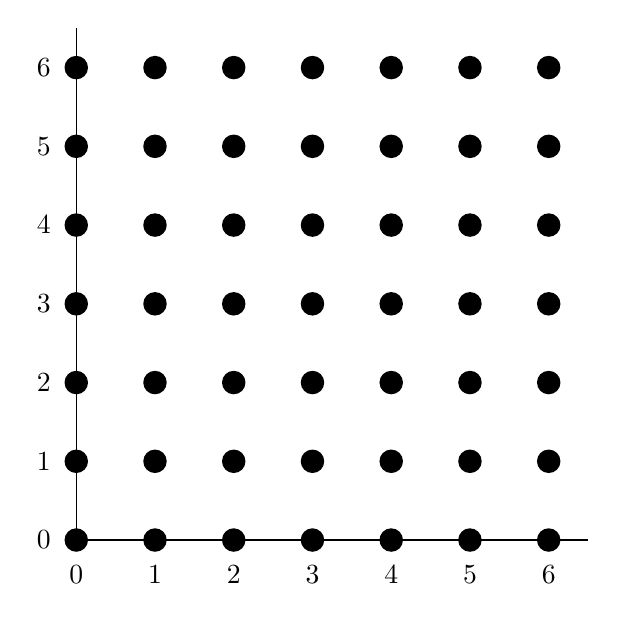
\begin{tikzpicture}[scale=1]
        \foreach \x in {0,...,6}
            {
                \foreach \y in {0,...,6}
                    {
                        \node at (\x, \y)[circle,fill,inner sep=3pt]{};
                    }
                \node[left] at (-0.2, \x){$\x$};
                \node[below] at (\x, -0.2){$\x$};
            }

        \draw (0.0, 0.0) -- (6.5, 0.0);
        \draw (0.0, 0.0) -- (0.0, 6.5);
    \end{tikzpicture}
\end{center}
这个平面上的``点阵''被称为\emph{格 (Lattice)}。现在有一个有趣的问题:在格中,给定任意一点,从原点 $(0, 0)$ 到该点有多少条路径?让我们具体说明一下。我们将\textbf{格路径}定义为从 $(0, 0)$ 到特定点的路径,并且在每一步中只能\emph{向右}或\emph{向上}移动。下面的定义详细说明了这一点:

\begin{definition}
    设 $(x,y) \in (\mathbb{N} \cup \{0\})^2$。到 $(x, y)$ 的\dotuline{格路径}是二维格中的一个有序格点元组,其中该元组的第一个元素为 $(0, 0)$,最后一个元素为 $(x, y)$,并且元组中的每个元素与前一个元素相比,只有一个坐标增加了正好一个单位。

    更严格地说,给定 $(x, y)$,格路径是 $n \in \mathbb{N}$ 元组 $(P_1, P_2, \dots, P_n)$,其中每个 $P_i = (x_i, y_i)$ 是格中的一个点,并且
    \[\forall i \in [n - 1] \centerdot \big((x_{i+1}, y_{i+1}) = (x_i + 1, y_i)\big) \lor \big((x_{i+1}, y_{i+1}) = (x_i, y_i + 1)\big)\]
    此外,$(x_1, y_1) = (0, 0)$ 且 $(x_n, y_n) = (x, y)$。

    也就是说,格路径是从 $(0, 0)$ 到 $(n, n)$ 的一系列格点,其中我们每一步只允许向右或向上移动一个格点。
\end{definition}

\begin{example}
    考虑二维格中的格点 $(2,4)$。如下图所示,我们展示了几条到 $(2,4)$ 的格路径。

    \begin{center}
        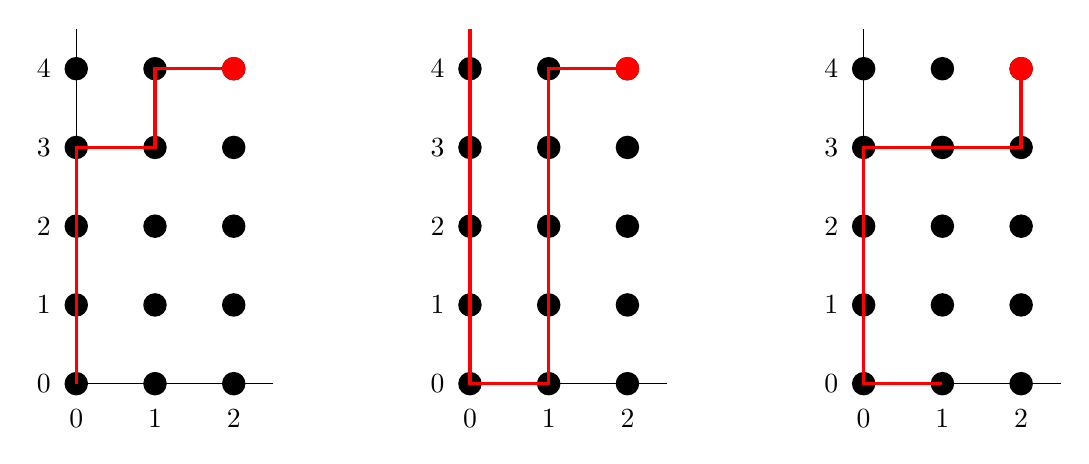
\begin{tikzpicture}[scale=1]
            \foreach \n in {0,5,10}
                {
                    \foreach \x in {0,...,2}
                        {
                            \foreach \y in {0,...,4}
                            \node at (\x+\n, \y)[circle,fill,inner sep=3pt]{};

                            \node[below] at (\x+\n, -0.2){$\x$};
                        }
                    \foreach \y in {0,...,4}
                    \node[left] at (\n-0.2, \y){$\y$};

                    \draw (\n, 0.0) -- (2.5+\n, 0.0);
                    \draw (\n, 0.0) -- (\n, 4.5);
                    \node[red] at (\n+2.0, 4.0)[circle,fill,inner sep=3pt]{};
                }
            \draw[red, very thick] (0.0, 0.0) -- (0.0, 3.0) -- (1.0, 3.0) -- (1.0, 4.0) -- (2.0, 4.0);
            \draw[red, very thick] (5.0, 4.5) -- (5.0, 0.0) -- (6.0, 0.0) -- (6.0, 4.0) -- (7.0, 4.0);
            \draw[red, very thick] (11.0, 0.0) -- (10.0, 0.0) -- (10.0, 3.0) -- (12.0, 3.0) -- (12.0, 4.0);
        \end{tikzpicture}
    \end{center}

    我们的问题是:

    \begin{quotation}
        给定 $(a,b) \in (\mathbb{N} \cup \{0\})^2$,从原点到 $(a, b)$ 有多少条\emph{不同的}格路径?
    \end{quotation}

    为了回答这个问题,我们先来看一个简单的例子,使用较小的数值,这样我们可以枚举出所有的路径。假设我们要找从 $(0, 0)$ 到 $(2, 2)$ 的格路径:

    \begin{center}
        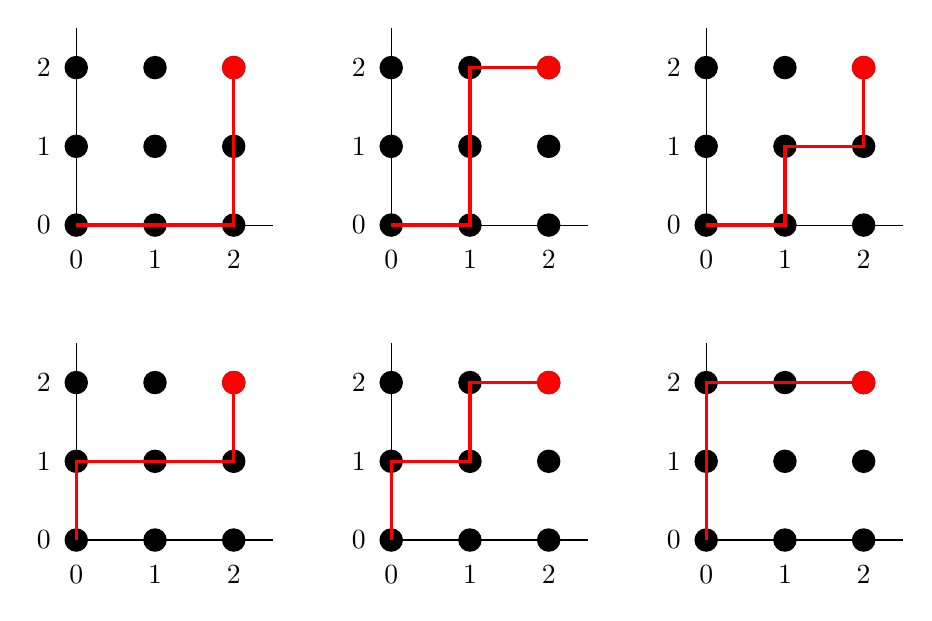
\begin{tikzpicture}[scale=1]
            \foreach \m in {0, 4}
                {
                    \foreach \n in {0, 4, 8}
                        {
                            \foreach \x in {0,...,2}
                                {
                                    \foreach \y in {0,...,2}
                                    \node at (\x+\n, \y+\m)[circle,fill,inner sep=3pt]{};

                                    \node[left] at (\n-0.2, \x+\m){$\x$};
                                    \node[below] at (\x+\n, \m-0.2){$\x$};
                                }

                            \draw (\n, \m) -- (2.5+\n, \m);
                            \draw (\n, \m) -- (\n, 2.5+\m);
                            \node[red] at (\n+2.0, \m+2.0)[circle,fill,inner sep=3pt]{};
                        }
                }
            \draw[red, very thick] (0.0, 0.0) -- (0.0, 1.0) -- (2.0, 1.0) -- (2.0, 2.0);
            \draw[red, very thick] (4.0, 0.0) -- (4.0, 1.0) -- (5.0, 1.0) -- (5.0, 2.0) -- (6.0, 2.0);
            \draw[red, very thick] (8.0, 0.0) -- (8.0, 2.0) -- (10.0, 2.0);

            \draw[red, very thick] (0.0, 4.0) -- (2.0, 4.0) -- (2.0, 6.0);
            \draw[red, very thick] (4.0, 4.0) -- (5.0, 4.0) -- (5.0, 6.0) -- (6.0, 6.0);
            \draw[red, very thick] (8.0, 4.0) -- (9.0, 4.0) -- (9.0, 5.0) -- (10.0, 5.0) -- (10.0, 6.0);
        \end{tikzpicture}
    \end{center}
    我们如何用\emph{组合的}方法来表示格路径呢?也就是说,怎样表示才能方便我们计数某些对象?想一想格路径的定义:在构建格路径的每一步中,每次``移动''都必须向右或向上。因此,用某种方式表示每次的``向右''移动和``向上''移动是有意义的。然后,我们只需要计算有多少种``向右''和``向上''选择的序列能把我们带到目标点 $(x, y)$。

    这其实很简单!平面上的点 $(x, y)$ 有什么特征呢?它在 $(0, 0)$ 的右边有 $x$ 个格点,并且在 $(0, 0)$ 的上方有 $y$ 个格点。因此,无论路径怎么走,我们都知道必须有 $x$ 次向右移动和 $y$ 次向上移动。回头看看上面到 $(2, 2)$ 的 $6$ 条格路径。想象一下沿着路径,从 $(0, 0)$ 开始,在每个格点上根据下一步的方向写下 $R$ 或 $U$。这样就得到了以下 $6$ 个由 $R$ 和 $U$ 组成的序列:
    \[RRUU \:,\: RUUR \:,\: RURU \:,\: URRU \:,\: URUR \:,\: UURR\]
    这些序列有什么共同特征呢?每个序列都有 $2$ 个 $R$ 和 $2$ 个 $U$,因为我们必须在 $(2,2)$ 结束,所以每个序列总共有 $4$ 项。注意,这很像一个受限字母表/单词问题:我们希望找到从字母表 $\{R,U\}$ 中抽取,长度为 $4$ 的单词的个数,并且每个字母恰好出现两次!

    通常情况下,我们知道到 $(x, y)$ 的任意格路径都可以表示为一个恰好包含 $x$ 个 $R$ 和 $y$ 个 $U$ 的 $(x + y)$-元组。为了确定有多少这样的序列,我们可以通过两步来确定:
    \begin{enumerate}
        \item 从 $x + y$ 个空位中选择 $x$ 个填充 $R$:有 $\big({x+y \atop x}\big)$ 种方式
        \item 用 $U$ 填充剩下的 $(x + y) - x = y$ 个空位:这种情况只有 $1$ 种确定的填充方式
    \end{enumerate}
    因此,我们得到如下结论。

    \begin{proposition}
        对于每个 $(x,y) \in (\mathbb{N} \cup \{0\})^2$,从 $(0,0)$ 到 $(x,y)$ 恰好有 $\begin{pmatrix}
                x+y \\x
            \end{pmatrix}$ 条格路径。
    \end{proposition}

    我们将在练习中探索格路径的一些有趣的应用和性质。目前,我们想强调它们的存在及其与序列和选择之间的关系。但这里还有一个有趣的观察:为什么我们选择计算长度为 $x+y$ 的序列中恰好有 $x$ 个 $R$ 的数量?计算长度为 $x+y$ 的序列中恰好有 $y$ 个 $U$ 的数量会有什么不同吗?想一想:每条到 $(x, y)$ 的格路径需要恰好 $x$ 个 $R$ 和 $y$ 个 $U$,确保其中一个属性成立也就保证了另一个属性的成立。因此,我们可以得出以下结论:

    \begin{proposition}
        对于每个 $(x,y) \in (\mathbb{N} \cup \{0\})^2$,从 $(0,0)$ 到 $(x,y)$ 恰好有 $\begin{pmatrix}
            x+y \\y
        \end{pmatrix}$ 条格路径。
    \end{proposition}

    这不仅证明了如下事实
    \[\begin{pmatrix}x+y \\x\end{pmatrix} = \begin{pmatrix}x+y \\y\end{pmatrix}\]
    而且也向我们介绍了一种新的有用的证明策略:\textbf{两法计数}。我们确定了一组对象(从 $(0, 0)$ 到 $(x, y)$ 的格路径集合),并解释了两种\emph{不同的}计数方法。每种方法都得到了该集合基数的不同表达式,因此我们可以确定这两个表达式是相等的。这个例子展示了两法计数的主要思想,我们将在下一节中探讨更多例子和这一技术的应用。
\end{example}